\subsection{HTB04 - Friendzone}

    \subsubsection{Escaneo}
        \large{Como primera etapa de la Prueba de Penetración realizamos un escaneo de puertos abiertos en la máquina víctima con la herramienta "Nmap", donde se encuentran siete de ellos.}
        \par
        \begin{figure}[h!]
            \centering
            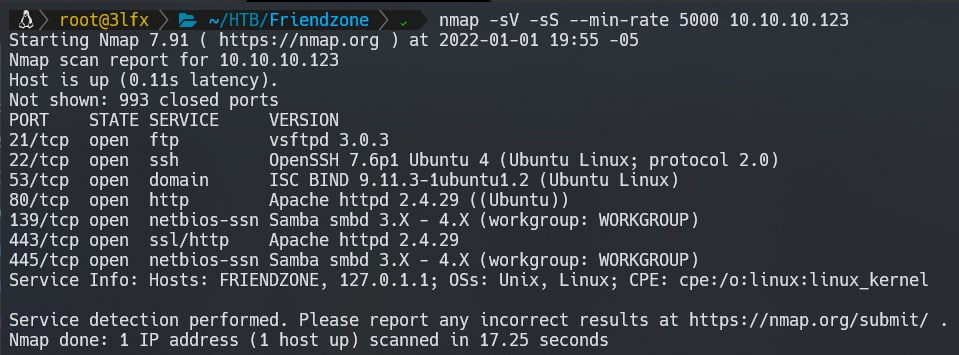
\includegraphics[width=0.99\textwidth]{informe4/imagenes/friendzone/01_escaneo.png}
            \caption{Escaneo de puertos Friendzone} 
        \end{figure}  

    \subsubsection{Análisis de Vulnerabilidades}

    \subsubsection{Explotación}

    \subsubsection{Escalamiento de Privilegios}

    \subsubsection{Post-Explotación}

    \subsubsection{Recomendaciones de Mitigación}
